\documentclass[border=10pt]{standalone}
\usepackage[svgnames]{xcolor}
\usepackage{amsmath}
\usepackage{pgfplots}
\pgfplotsset{compat=newest}
\usepackage[sfdefault]{FiraSans}
\usepackage{FiraMono}
\renewcommand*\familydefault{\sfdefault}
\begin{document}
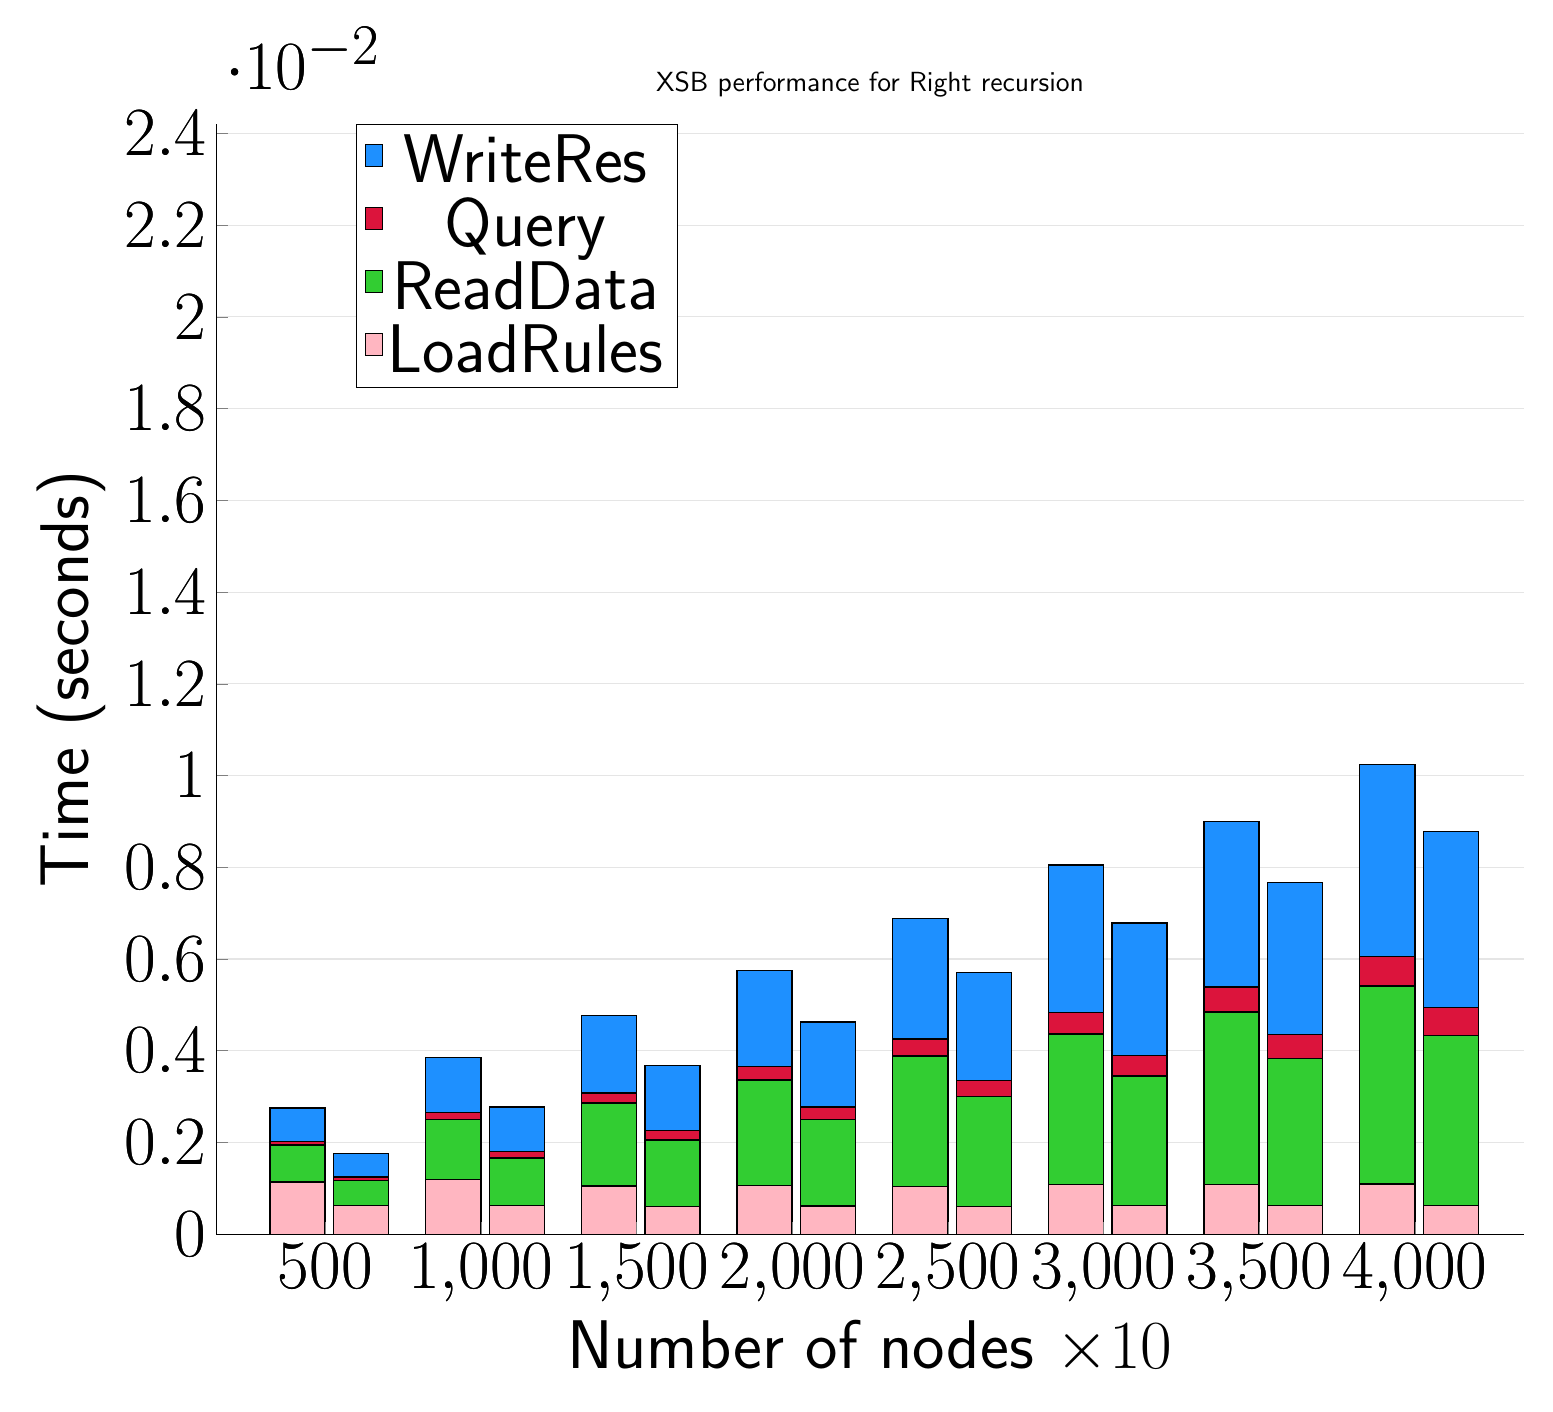
\begin{tikzpicture}
\begin{axis}[
   ybar stacked,
   title={XSB performance for Right recursion},
   bar shift=-10pt,
   width=1.5\textwidth,
   bar width=0.7cm,
   ymajorgrids, tick align=inside,
   major grid style={draw=gray!20},
   xtick=data,
   ymin=0, ymax=0.024215764999389648,
   axis x line*=bottom,
   axis y line*=left,
   enlarge x limits=0.1,
   legend style={
       at={(0.23, 1)},
       anchor=north,
       legend columns=1,
       font=\Huge,
   },
   ylabel={Time (seconds)},
   xlabel={Number of nodes $\times 10$},
   label style={font=\Huge},
   tick label style={font=\Huge},
]
\addlegendimage{fill=DodgerBlue, draw=black, line width=0.2pt}
\addlegendentry{WriteRes}
\addlegendimage{fill=Crimson, draw=black, line width=0.2pt}
\addlegendentry{Query}
\addlegendimage{fill=LimeGreen, draw=black, line width=0.2pt}
\addlegendentry{ReadData}
\addlegendimage{fill=LightPink, draw=black, line width=0.2pt}
\addlegendentry{LoadRules}
\addplot +[fill=LightPink, draw=black, line width=0.5pt] coordinates {
    (500, 0.001134371757507325)
    (1000, 0.001186513900756836)
    (1500, 0.001047325134277344)
    (2000, 0.001066899299621582)
    (2500, 0.00104498863220215)
    (3000, 0.0010851621627807622)
    (3500, 0.0010828971862792969)
    (4000, 0.001092243194580079)
};
\addplot +[fill=LimeGreen, draw=black, line width=0.5pt] coordinates {
    (500, 0.0008097171783447271)
    (1000, 0.001314949989318848)
    (1500, 0.001814985275268556)
    (2000, 0.00229659080505371)
    (2500, 0.002838587760925294)
    (3000, 0.0032788991928100588)
    (3500, 0.0037578344345092795)
    (4000, 0.004317927360534666)
};
\addplot +[fill=Crimson, draw=black, line width=0.5pt] coordinates {
    (500, 7.936954498291015e-05)
    (1000, 0.0001534223556518555)
    (1500, 0.0002190589904785156)
    (2000, 0.0002898931503295898)
    (2500, 0.00037460327148437507)
    (3000, 0.00047132968902587893)
    (3500, 0.0005513191223144533)
    (4000, 0.000649714469909668)
};
\addplot +[fill=DodgerBlue, draw=black, line width=0.5pt] coordinates {
    (500, 0.0007289409637451172)
    (1000, 0.0012006998062133783)
    (1500, 0.0016900062561035164)
    (2000, 0.0021021366119384774)
    (2500, 0.002625608444213866)
    (3000, 0.0032145977020263663)
    (3500, 0.003607249259948729)
    (4000, 0.004184317588806155)
};
\end{axis}
\begin{axis}[
   ybar stacked,
   bar shift=13pt,
   width=1.5\textwidth,
   bar width=0.7cm,
   ymajorgrids, tick align=inside,
   major grid style={draw=none},
   xtick=data,
   ymin=0, ymax=0.024215764999389648,
   axis x line*=none,
   axis y line*=none,
   enlarge x limits=0.1,
   label style={font=\Huge},
   tick label style={font=\Huge},
]
\addplot +[fill=LightPink, draw=black, line width=0.5pt] coordinates {
    (500, 0.0006251)
    (1000, 0.0006293999999999998)
    (1500, 0.0006049000000000003)
    (2000, 0.0006117000000000004)
    (2500, 0.0006043000000000005)
    (3000, 0.0006246000000000002)
    (3500, 0.0006211999999999998)
    (4000, 0.0006276999999999996)
};
\addplot +[fill=LimeGreen, draw=black, line width=0.5pt] coordinates {
    (500, 0.0005511999999999993)
    (1000, 0.0010302000000000002)
    (1500, 0.0014505)
    (2000, 0.0018939999999999999)
    (2500, 0.0023967)
    (3000, 0.0028251)
    (3500, 0.0032141)
    (4000, 0.0037044)
};
\addplot +[fill=Crimson, draw=black, line width=0.5pt] coordinates {
    (500, 7.300000000000047e-05)
    (1000, 0.0001425999999999994)
    (1500, 0.00020650000000000009)
    (2000, 0.0002692999999999994)
    (2500, 0.00035010000000000087)
    (3000, 0.0004404000000000008)
    (3500, 0.0005193999999999996)
    (4000, 0.0006082000000000004)
};
\addplot +[fill=DodgerBlue, draw=black, line width=0.5pt] coordinates {
    (500, 0.0005166999999999992)
    (1000, 0.0009725000000000008)
    (1500, 0.0014221999999999998)
    (2000, 0.0018493000000000006)
    (2500, 0.0023594999999999996)
    (3000, 0.0028949999999999996)
    (3500, 0.0033131000000000002)
    (4000, 0.003845)
};
\end{axis}
\end{tikzpicture}

\end{document}
